\Subsubsubsection{Sensores}

%%%%%%TEMPERTURA%%%%%%
Para el sensor de temperatura la primer opción a descartar es aquella que no cumple con el rango de temperaturas a medir, por lo que el Ds18b20 queda descartado a pesar de su bajo costo. Luego, de las opciones que quedan, todas son de un costo similar, sin embargo hay que tener en cuenta que para la termocupla se debe proporcionar una manera de medir la temperatura de referencia, la cual puede ser tanto una RTD como un IC, aumentando el costo de la termocupla. Tanto la TC como la RTD necesitan un circuito convertidor para poder medir directamente el valor de la temperatura con un micro controlador, mientras que los IC ofrecen directamente una salida digital.% La mejor precisión de la medición se da con una RTD, seguido por los IC y finalmente la TC.

Una desventaja de la TC es que tiende a envejecer rápidamente. Si bien el dispositivo no se usará más de 3 meses seguidos, este podrá ser reutilizado, dándole mayor peso al factor del envejecimiento. El autocalientamiento también es contraproductivo en la medición de temperatura debido a que este puede alterar la misma si no es tenido en cuenta. Las TC no cuentan con este inconveniente debido a su principio de funcionamiento, mientras que con las otras opciones si lo es. Con la RTD este efecto depende directamente con la corriente que se suministra para la medición, y con los IC es un aspecto que es considerado por los diseñadores de los mismos.

Por estas razones los candidatos a terminan siendo DHT-22 y la PT-100. Un punto favorable para la DHT-22 es que no necesita un circuito extra. Adicionalmente esta unidad cuenta con una medición de humedad, lo que brinda la posibilidad de usarlo también para dicha variable o como un complemento de otro sensor.

%%%%%%HUMEDAD%%%%%%
En la elección para la medición de humedad, como primer criterio, se busca que pueda medir el rango entero de la humedad relativa y que cuente con una precisión considerable. Dadas estas consideraciones, se descarta el DHT-11 y AM-1001. Es así que de los dos restantes, se opta por el DHT-22 debido a que por un menor costo se obtienen mejores prestaciones. Teniendo en cuenta esto se utilizará tanto para la medición de temperatura y humedad el DHT-22.


%%%%%%LUMINSIDAD%%%%%%
En cuanto a la luminosidad, principalmente se deberá asegurar el funcionamiento en el rango de temperatura en el cual operará el dispositivo, por lo cual el OPT-101 queda descartado. Además, se tiene en cuenta la potencia utilizada, el rango de medición de los sensores y el tipo de alimentación.

La comunicación puede ser analógica en corriente para el TEMT-6000, pero este necesitará un amplificador de corriente o un convertidor para esta corriente a un nivel medible.

Existen también otros sensores que tienen una salida analógica de tensión como el GL55-LM393 con un rango entre 0 y $V_{dd}$. Este también provee con una salida digital, pero esta funciona como un schmitt trigger.

Por último el BJ-1750 cuanta con una salida digital con el protocolo de comunicación I2C. Teniendo en cuenta esto se opta por utilizar este último sensor. 

Luego para el modulo RTC se tom\'o un  m\'odulo que tenga I2C, y que cuyo rango de almimentacion se encuentre entre 3.3 y 5 V, por lo que se opta por el DS3231.
%%%%%%IAMGENES%%%%%%
Finalmente, para la cámara que obtendrá las imágenes, se tuvo en cuenta fundamentalmente la relación precio-resolución de la cámara, al igual que la integración con Linux y el factor de contar con una API para el lenguaje C. Por lo que la RPi-CMOD-V2 fue la cámara seleccionada.


\Subsubsubsection{Almacenamiento}

El factor principal para seleccionar la memoria SD a utilizar es el rango de temperaturas de operación. Es por este factor que se elije la SDSDQAF3-XI, ya que esta se encuentra en un rango seguro (mayor a las demás).

Dado que se recolectará un volumen de datos del que no se tiene una gran certeza, debido a que una parte será lo que provenga de la mochila, se estima en función de los datos del nido y del periodo de activación de los sensores, que una memoria de 16 GBy es suficiente incluso si aumenta el volumen de datos.

\Subsubsubsection{Unidades de procesamiento}

Para este módulo se opta por la Raspberry Pi 3B, ya que posee Bluetooth BLE (Bluetooth Low Energy), es el dispositivo más económico, más pequeño y cuenta con soporte para micro SD.

En cuanto las temperaturas de funcionamiento, este dispositivo se encuentra dentro del rango necesario. Además, los módulos Raspberry Pi trabajan entre 20 °C y 30 °C por encima de la temperatura ambiente debido a su autocalentamiento. También es sabido que los integrados R-Pi pueden llegar a soportar temperaturas extremas, tales como las que se dan en la Antártida \cite{ref:Penguin}.

Además, este dispositivo seleccionada se caracteriza por ser compatible con la cámara seleccionada sin  de adaptadores.

\Subsubsubsection{Comunicación}

En cuanto a la comunicación se utilizará BLE para la conexión con el ave, y WiFi para la comunicación con un tercero.
Ambos de estos se encuentran disponibles para su uso en el módulo Raspberry Pi 3B.


\Subsubsubsection{Batería}

La batería a emplear queda determinada en función del consumo del sistema y de la energía que se deba almacenar en caso de emergencias. 

Los consumos de potencia de las partes del sistema se detallan en la Sección \ref{sec:calc_potencias}.

De esta forma, para alimentar tanto a los sensores como a la R-Pi en un día se requieren $151.2 \ kJ$. Con una batería de $21 \ Ah$ de capacidad se consigue la especificación mencionada, por lo que se opta por la batería UL24-12 de Ultracell ya que la batería de Probattery es mucho más pesada.

Cabe notar que los $24 \ Ah$ de la batería seleccionada son nominales, por lo que se debe calcular la capacidad real (la cual será ligeramente menor debido a condiciones del entorno y calidad de esta). Para obtener la capacidad real de la batería se utiliza la información proporcionada en la hoja de datos. En la Figura (\ref{fig:ctemp}) se puede observar como a una temperatura de trabajo de $10°C$ y una razón de descarga de $0.05CA$ (descarga total en $20 \ hs$) la capacidad efectiva restante de la batería es del $90\% $. Por otro lado, en la Figura (\ref{fig:cdod}) se observa como teniendo en cuenta una vida útil de $540$ ciclos (es decir, 2 años de uso ininterrumpido) la capacidad efectiva restante sigue siendo del $100\%$.
 
\begin{figure}[H]
	\centering
	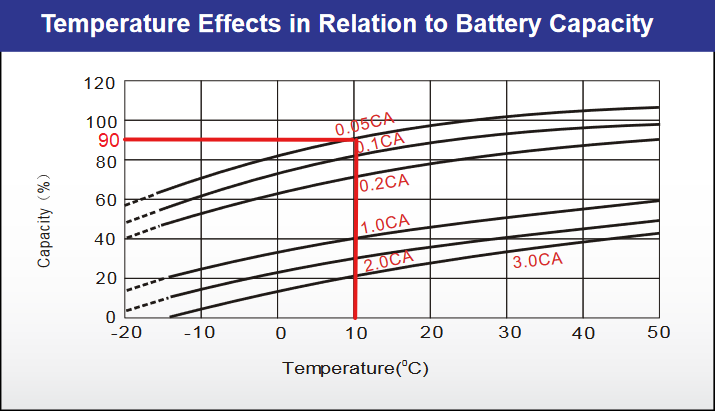
\includegraphics[width=0.9\linewidth]{ImagenesFactibilidad/UL24-12_Ctemp}
	\label{fig:ctemp}
	\caption{Efectos de la temperatura en relación a la capacidad de la batería.}
\end{figure}

\begin{figure}[H]
	\centering
	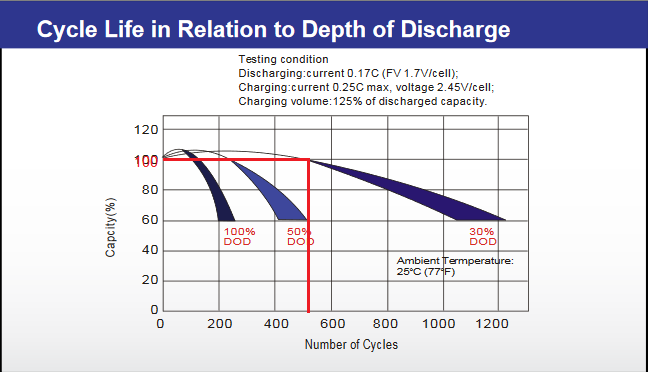
\includegraphics[width=0.9\linewidth]{ImagenesFactibilidad/UL24-12_Cdod}
	\label{fig:cdod}
	\caption{Ciclos de vida en relación a la profundidad de descarga.}
\end{figure}

Por ende, la capacidad efectiva, calculada como:
\begin{equation}
C_{ef} = C_{nom}*0.9*1 = 21.6 \ Ah
\end{equation}

por lo que la batería elegída sería apta para el proyecto.

\Subsubsubsection{Alimentación}

Para poder abastecer a la batería seleccionada, con un panel $23.1 \ W$ se puede proveer la potencia requerida.

En cuanto a la etapa de carga, para el cargador MPPT de la batería principal se optó por la DFR0580 debido al precio, la documentación clara y la tecnología de la batería a usar.
